\section{Anwendungsszenario 2: Hindernisdetektion}
Im nächsten Schritt wird der Fall betrachtet, dass der Weg des Roboters durch ein unbekanntes Hindernis versperrt wird. Darunter ist ein Objekt zu verstehen, dass bei der Kartenaufzeichnung nicht vorhanden war, weshalb der Roboter auf seine Sensordaten zurückgreifen muss, um den Gegenstand zu detektieren und in die Wegplanung einzuarbeiten. In der folgenden Abbildung sind die Position des Roboters als auch die aktuellen Sensordaten zu erkennen. An letzteren lässt sich die Position des Hindernisses deutlich erkennen.
\begin{figure}[!ht]
\centering
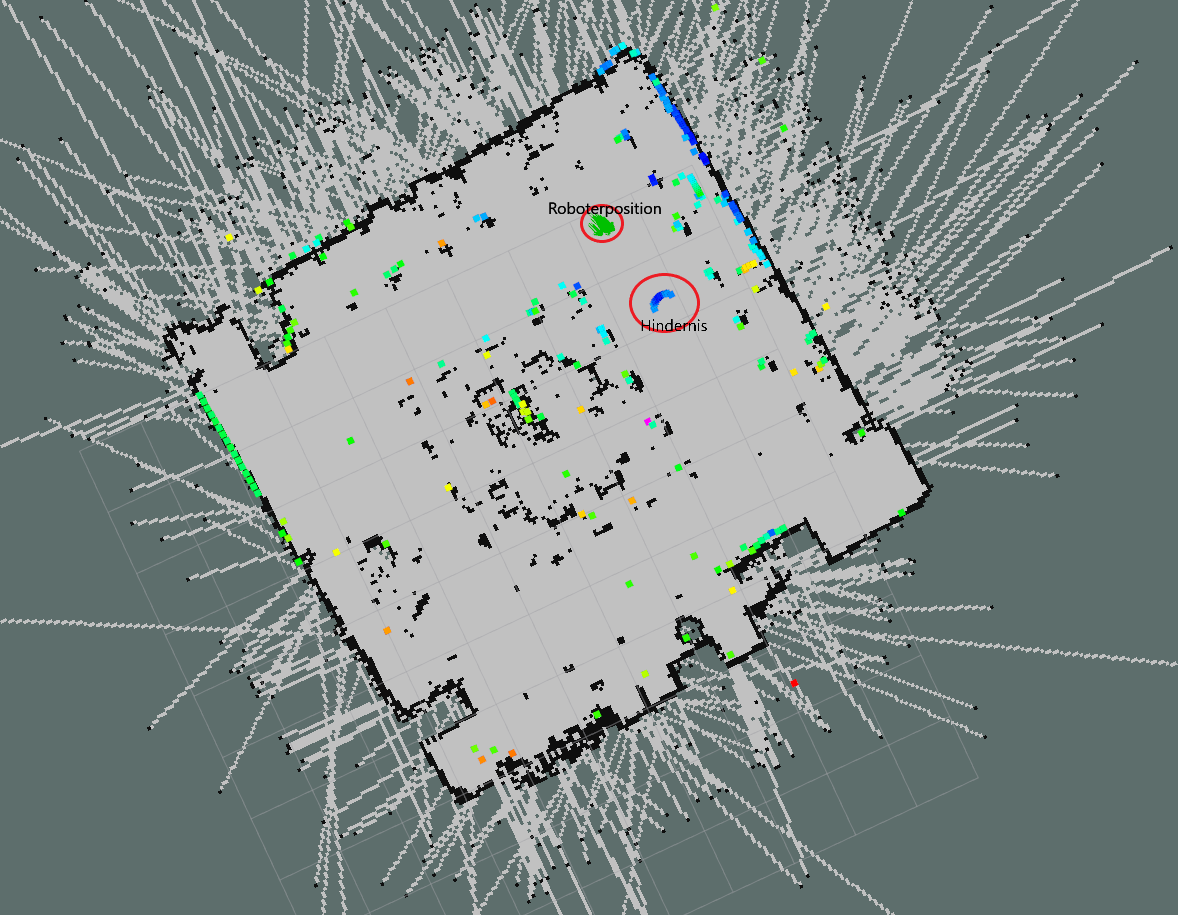
\includegraphics[scale=0.9,trim={13cm 13cm 9cm 2cm},clip]{img/Experiment2_Laserscan_Hindernis.png}
\caption{Roboter und Sensordaten mit Hindernis}
\end{figure}
\newpage
Die beiden weiteren Abbildungen zeigen wie die Sensordaten in die globale Kostenkarte integriert werden und wie daraufhin der globale Plan um die Distanzmessungen herumführt.
\begin{figure}[!ht]
\centering
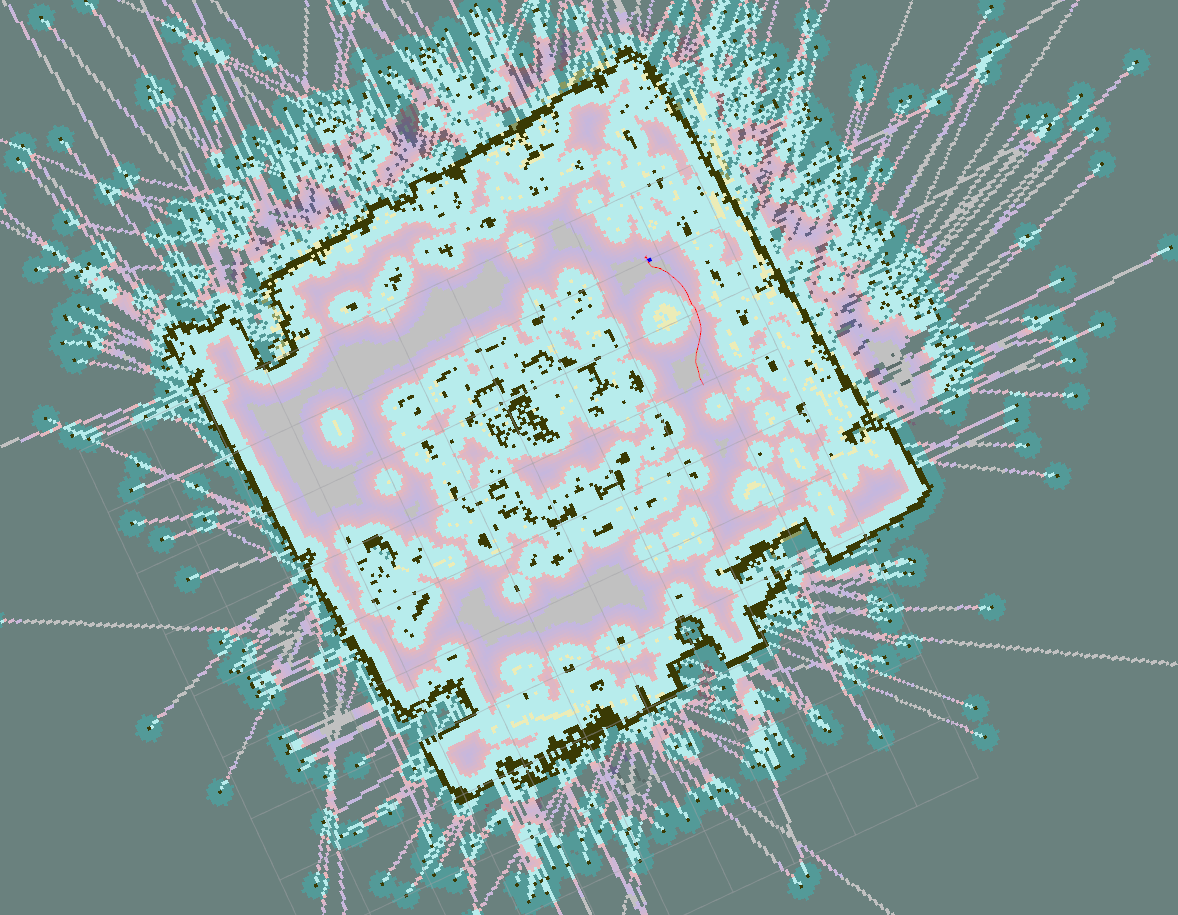
\includegraphics[width=0.45\linewidth ,trim={13cm 11cm 9cm 2cm},clip]{img/Experiment2_Global_Plan_Hindernis.png}
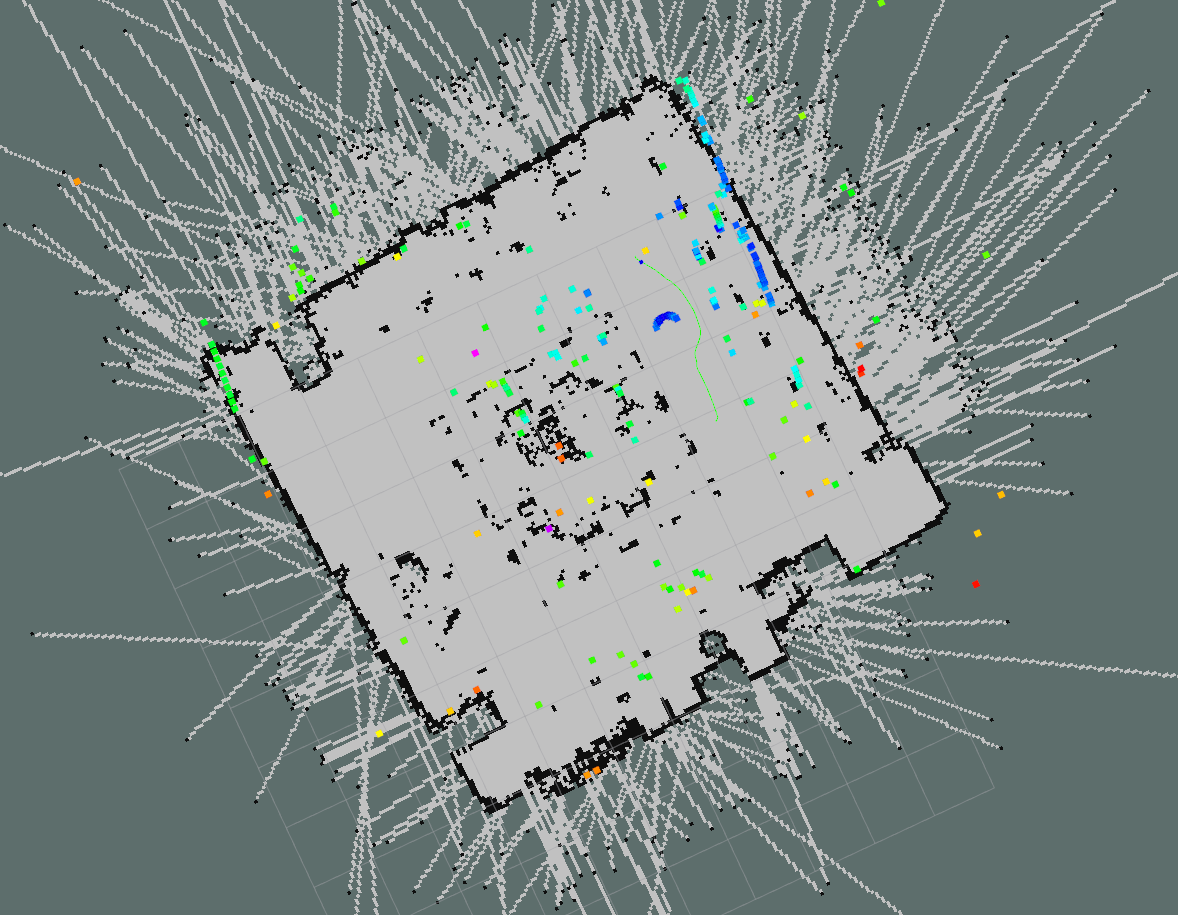
\includegraphics[width=0.45\linewidth ,trim={13cm 11cm 9cm 2cm},clip]{img/Experiment2_Global_Plan_Lascerscan_Hindernis.png}
\caption{Integration der Sensordaten in die Pfadplanung}
\end{figure}

In dem Experiment hat der Roboter das Hindernis nicht nur erfolgreich erkannt und in die Planung aufgenommen, sondern konnte die Route auch abfahren. Allerdings wurde hierbei die Geschwindigkeit deutlich reduziert, was darauf zurückzuführen ist, dass der Plan nach wie vor durch suboptimale Zonen führt. Der Grund hierfür liegt darin, das keine alternative Route zum Ziel führt, was aber auch zur Folge hat, dass der lokale Planer die Geschwindigkeit des Roboters reduziert, um auf potentielle Kollisionen reagieren zu können.